\section{Marco teórico}
        \subsection{Hamming}
        La red Hamming es una arquitectura capaz de reconocer patrones binarios. Está formada por dos capas como se muestra en la figura \ref{fig:hamming-diagrama}. La primera capa es una capa de propagación hacia adelante (feedforward en ingles), esto quiere decir que los datos de entrada solamente pueden avanzar de su entrada a la salida de la red nunca en sentido opuesto.
        La expresión correspondiente a esta capa es la siguiente.
        \[ a^1=purelin(W^1p+b^1) \]
        donde $a^1$ es la salida de la capa, $W^1$ es la matriz de pesos, $p$ es el vector de entrada y $b^1$ es el bias.
        \begin{figure}[H]
            \begin{center}
                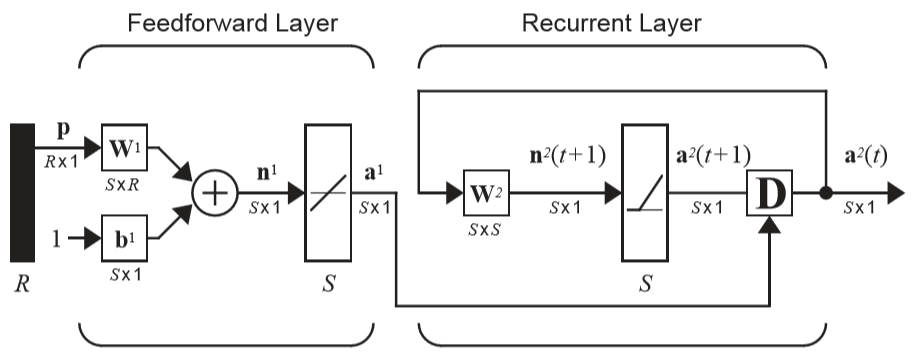
\includegraphics[width=16cm]{img/hamming/diagrama.png}
                \caption{Estructura de la red de Hamming. \cite{libro1}}
                \label{fig:hamming-diagrama}
            \end{center}
        \end{figure}
        En la siguiente capa, la capa recurrente, es donde se realiza una competición con la cual se puede determinar que vector prototipo es el más parecido al vector de entrada.\cite{libro1}
        Es por esto que esta red es de tipo competitiva además de que es de las redes más simples en su categoría.
        Esta capa tiene como expresión matemática a:
        \[\boldsymbol{a^2(t+1) = poslin(W^2a^2(t))}\]
        En esta capa se produce una inhibición lateral, esto quiere decir que la salida de cada neurona tiene un efecto inhibitorio sobre el resto de las neuronas lo cual se ve reflejado en el funcionamiento de la red donde a medida que avanza el valor de alguna neuronas disminuye más lento que el resto. \cite{libro1} 
        
        La construcción de una red de Hamming que reconozca un grupo de vectores prototipo es la siguiente:
        \begin{enumerate}
            \item Si tenemos un conjunto de vectores prototipo como el siguiente.
            \[ \left\lbrace \boldsymbol{p_1, p_2, ..., p_Q} \right\rbrace  \]
            La transpuesta de estos vectores sirven para llenar la matriz de pesos de la primera capa $W^1$ de la siguiente forma.
            \[\boldsymbol{ W^{1}} = \left[\begin{array}{c}\boldsymbol{p^{T}_1}\\\boldsymbol{ p^{T}_2}\\ \vdots \\ \boldsymbol{p^{T}_Q}\end{array}\right]  \]
            \item Por otro lado el bias es llenado con el tamaño $R$ de los vectores prototipo, es decir,
            \[ b^{1} = \left[\begin{array}{c}R\\ R\\ \vdots \\ R\end{array}\right] \]
            \item Para la siguiente capa debido a que es una capa recurrente debemos de inicializar la capa recurrente con el valor de salida de la capa feedforward, es decir, $\boldsymbol{a^2(0) = a^1}$, esto con el fin de poder obtener los siguientes valores de la forma $\boldsymbol{a^2(t+1) = poslin(W^2a^2(t))}$.
            \item Lo siguiente es llenar la matriz de pesos de la segunda capa en donde los elementos en la diagonal de la matriz tendrán valores de uno y el resto serán valores pequeños negativos.
            \[ w^2_{i,j} = \begin{cases} 1 & i=j \\-\epsilon & \text{en otro caso} \end{cases} \]
            El valor de épsilon se obtiene por la siguiente formula: $ 0 < \epsilon <\frac{1}{S-1}$ donde $S$ es el número de neuronas
            \item Finalmente, solo se tiene que introducir un vector en la entrada de la primera capa, propagar hacia adelante y utilizar la recurrencia de la segunda capa hasta que solo una salida de esta capa tenga un valor positivo, el indice de la salida indica que vector prototipo reproduce dicha salida.
        \end{enumerate}
    \newpage
        \subsection{Perceptron}
        El perceptron fue desarrollado en los años cincuenta por un grupo de investigadores entre los que estaba Frank Rosenblantt, la principal característica de esta red es que utiliza un algoritmo de aprendizaje supervisado esto quiere decir que se le tiene que dar ejemplos de como operar (conjunto de entrenamiento), este conjunto de entrenamiento tiene la siguiente forma:
        \[ \left\lbrace \boldsymbol{p_1, t_1}\right\rbrace , \left\lbrace \boldsymbol{p_2, t_2}\right\rbrace , ... , \left\lbrace \boldsymbol{p_Q, t_Q}\right\rbrace  \]
        en donde cada par esta formado por un vector de entrada $\boldsymbol{p_q}$ y un vector objetivo $\boldsymbol{t_q}$ que es la salida correspondiente a dicho vector de entrada. \cite{libro1}
        Además, la arquitectura del perceptron es la siguiente:
        \begin{figure}[H]
            \begin{center}
                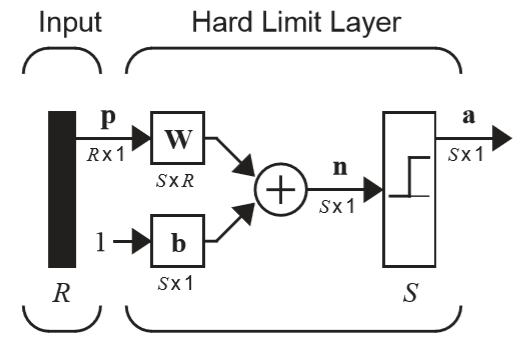
\includegraphics[width=8cm]{img/perceptron/perceptron.png}
                \caption{Arquitectura de un perceptron simple. \cite{libro1}}
                \label{fig:perpectron-diagrama}
            \end{center}
        \end{figure}
        Debido a que utiliza una función \emph{hardlim} la salida de la red solo puede tener dos posibles valores el cual esta definido por $\boldsymbol{a = hardlim(Wp+b)}$. El hecho de que solo tenga dos valores es lo que nos permite establecer una frontera de decisión entre dos clases como la de la figura \ref{fig:frontera}, esto en consecuencia de que cada neurona puede clasificar 2 diferentes clases.
        \begin{figure}[H]
            \begin{center}
                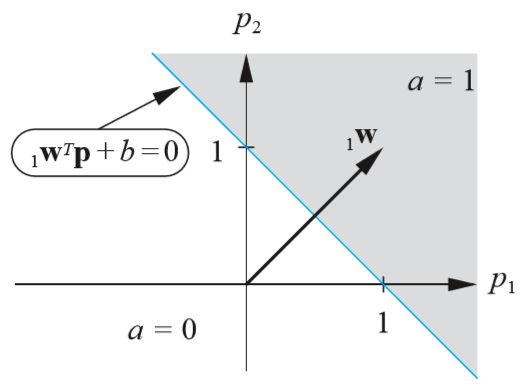
\includegraphics[width=8cm]{img/perceptron/frontera.png}
                \caption{Ejemplo de una frontera de decisión. \cite{libro1}}
                \label{fig:frontera}
            \end{center}
        \end{figure}
        Dicha frontera es determinada por un valor de entrada para el cual la salida de la red es 0, es decir,
        \[\boldsymbol{Wp+b} = 0 \]
        Como se menciono antes, el perceptron utiliza una regla de aprendizaje que se basa en la modificación de los pesos y bias con base a un error a lo largo de la propagación hacia adelante que se realiza. 
        Para lograr esto se sigue el siguiente algoritmo.
        \begin{enumerate}
            \item Se tiene el conjunto de entrenamiento
            \[ \left\lbrace \boldsymbol{p_1, t_1}\right\rbrace , \left\lbrace \boldsymbol{p_2, t_2}\right\rbrace , ... , \left\lbrace \boldsymbol{p_Q, t_Q}\right\rbrace\]
            \item Se inicializan los valores de $\boldsymbol{W}$ y $\boldsymbol{b}$ con valores aleatorios pequeños.
            \item Procedemos a hacer la propagación hacia adelante de un vector prototipo, es decir, evaluamos un $\boldsymbol{p_Q}$ en nuestra red de la forma.
            \[ \boldsymbol{a = hardlim(Wp_Q+b)} \]
            \item Lo siguiente es obtener el error comparando el valor objetivo asociado a dicho vector prototipo con la salida producida por la red
            \[ \boldsymbol{e=t-a} \]
            \item A continuación aplicamos el aprendizaje correspondiente al bias y matriz de pesos de nuestra red. Es decir, el nuevo valor de nuestra matriz de pesos sera igual al valor actual más el producto del error obtenido en el paso por la transpuesta del vector de entrada que se utilizo.
            \[ \boldsymbol{W^{nueva} = W^{vieja} + ep^{t}} \]
            Para el caso del bias tenemos algo similar solo que el nuevo valor de $\boldsymbol{b}$ sera igual al valor actual más el error producido.
            \[ \boldsymbol{b^{nueva} = b^{vieja} + e} \]
            \item Esto se realiza para cada elemento del conjunto de entrenamiento para poder completar una iteración.
            \item Este procedimiento se realiza hasta que cada salida de la red con cada vector de entrada sea igual a su correspondiente objetivo $a_Q = t_Q$ o en el caso de que se alcance un máximo de iteraciones.
        \end{enumerate}
        \newpage
        \subsection{ADALINE}
        La red ADALINE (ADAptive LInear NEuron) es muy similar a al perceptron con la diferencia que la función de transferencia es lineal en lugar de ser escalón esto se puede observar en la figura \ref{fig:adaline-diagrama}, y al igual que el perceptron solo pueden resolver problemas linealmente separables como por ejemplo el problema de la compuerta AND de la figura \ref{fig:AND}. \cite{pagina}
        \begin{figure}[H]
            \begin{center}
                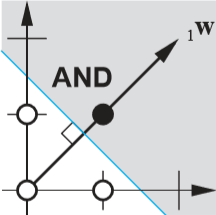
\includegraphics[width=5cm]{img/adaline/AND.png}
                \caption{La compuerta AND es linealmente separable. \cite{libro1}}
                \label{fig:AND}
            \end{center}
        \end{figure}
        Por otro lado un problema linealmente no separable seria el de la figura \ref{fig:XOR} ya que no es posible trazar lineas que funjan como frontera de decision entre las dos clases que tenemos.
        
        Otro aspecto importante de ADALINE es que el algoritmo LMS es mas poderoso que la regla de aprendizaje del perceptron. Esto debido a que la regla de aprendizaje del perceptron garantiza la convergencia a una solución que clasifica los vectores prototipo. Por lo que es sensible al ruido que se produce debido a que estos vectores suelen estar muy cerca de las fronteras de decisión.
        \begin{figure}[H]
            \begin{center}
                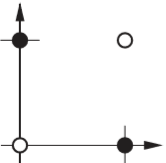
\includegraphics[width=5cm]{img/adaline/XOR.png}
                \caption{La compuerta XOR no se puede separar linealmente. \cite{libro1}}
                \label{fig:XOR}
            \end{center}
        \end{figure}
        Este problema es solucionado con LMS, el cual desplaza las fronteras de decisión lejos de los patrones de entrenamiento esto vuelve a este método más útil y aplicable a otros campos como el procesamiento de señales digital de señales en donde se utiliza para cancelar echo en las lineas telefónicas de larga distancia.
        
        La arquitectura de esta red es la siguiente.
        \begin{figure}[H]
            \begin{center}
                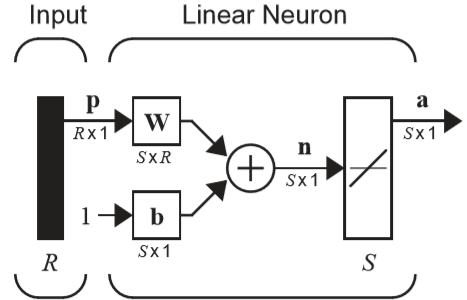
\includegraphics[width=9cm]{img/adaline/arquitectura.png}
                \caption{Arquitectura de la red ADALINE. \cite{libro1}}
                \label{fig:adaline-diagrama}
            \end{center}
        \end{figure}
        Se puede apreciar su similitud con el perceptron incluso en la ecuación que produce la salida de la red, la cual está definida como.
        \[ \boldsymbol{a = purelin(Wp+b)} \]
        Esta red es entrenada por aprendizaje supervisado por lo que utilizamos un conjunto de entrenamiento y el algoritmo LMS que se encarga de ajustar los pesos y bias con el objetivo de minimizar el error medio cuadrático.
        \[ \left\lbrace \boldsymbol{p_1, t_1}\right\rbrace , \left\lbrace \boldsymbol{p_2, t_2}\right\rbrace , ... , \left\lbrace \boldsymbol{p_Q, t_Q}\right\rbrace\]
        El algoritmo es el siguiente. \cite{otro}
        \begin{enumerate}
            \item Inicialización de los pesos y bias de forma aleatoria.
            \item Se aplica un patrón $p_Q$ de entrada.
            \item Se computa una salida lineal utilizando la red.
            \item Se calcula el error cometido por la red para dicho patrón el cual se calcula de la siguiente forma.
            \[\boldsymbol{e_Q = t_Q - a_Q} \]
            donde $\boldsymbol{e_Q}$ es el error, $\boldsymbol{t_Q}$ es el vector objetivo y $\boldsymbol{a_Q}$ es la salida que produce la red.
            \item Se actualizan los pesos y bias utilizando el error obtenido en el paso anterior de la siguiente forma.
            \begin{gather*}
            \boldsymbol{W}(k+1) = \boldsymbol{W}(k) +2\alpha \boldsymbol{e}(k)\boldsymbol{p^T}(k) \\
            \boldsymbol{b}(k+1) =\boldsymbol{b}(k) + 2\alpha \boldsymbol{e}(k)
            \end{gather*}
            donde $\boldsymbol{W}(k+1)$ y $\boldsymbol{b}(k+1)$ son los nuevos valores de nuestros pesos y bias, $\boldsymbol{W}(k)$ y $\boldsymbol{b}(k)$ son los valores actuales, $\alpha$ es un factor de aprendizaje que suele tener valores muy pequeños para evitar modificaciones drásticas en los valores de la red y $\boldsymbol{p^T}(k)$ es la transpuesta de nuestro vector de entrada.
            \item Se repiten los pasos 2 a 5 para todos los patrones de entrenamiento.
            \item Después de esto termina una iteración y se calcula el error cuadrático medio, este error es calculado de la siguiente forma.
            \[ e^2 = \frac{1}{Q} \sum _{i=1}^{Q} e^2_i \]
            Si el error cuadrático medio es un valor reducido aceptable o hemos alcanzado un máximo de iteraciones terminamos el proceso, de lo contrario se vuelve al paso 2.
        \end{enumerate}
    \newpage